
%%%%%%%%%%%%%%%%%%%%%%% file typeinst.tex %%%%%%%%%%%%%%%%%%%%%%%%%
%
% This is the LaTeX source for the instructions to authors using
% the LaTeX document class 'llncs.cls' for contributions to
% the Lecture Notes in Computer Sciences series.
% http://www.springer.com/lncs       Springer Heidelberg 2006/05/04
%
% It may be used as a template for your own input - copy it
% to a new file with a new name and use it as the basis
% for your article.
%
% NB: the document class 'llncs' has its own and detailed documentation, see
% ftp://ftp.springer.de/data/pubftp/pub/tex/latex/llncs/latex2e/llncsdoc.pdf
%
%%%%%%%%%%%%%%%%%%%%%%%%%%%%%%%%%%%%%%%%%%%%%%%%%%%%%%%%%%%%%%%%%%%


\documentclass[runningheads,a4paper]{llncs}
\usepackage{amssymb}
\setcounter{tocdepth}{3}
%\usepackage[margin=2in]{geometry}

\usepackage[noend]{algpseudocode}
\usepackage{subfig} 
\usepackage{graphicx}
\usepackage{frame,caption}
\usepackage{amsmath}
\usepackage{eulervm}
\usepackage{fontenc}
\usepackage{mathrsfs}
\usepackage{multirow, enumitem, longtable, rotating,lipsum, scrextend}
\usepackage{array}
\usepackage{floatflt}
\usepackage{makecell}
\usepackage{xcolor,soul}
\sethlcolor{yellow}	
\usepackage{floatrow}
\usepackage{setspace}
\newcommand{\argmax}{\operatornamewithlimits{arg\,max}}

%\usepackage{url}
%\urldef{\mailsa}\path|{ouldouali, nicolas.sabouret}@limsi.fr
%\urldef{\mailsb}\path{rich@wpi.edu}
%\urldef{\mailsc}\path{hatem.dhouib@ensta-paristech.fr}
%\newcommand{\keywords}[1]{\par\addvspace\baselineskip


\begin{document}
	
	\mainmatter  % start of an individual contribution
	
	% first the title is needed
	\title{Effect of Interpersonal Power on Negotiation Strategies in Collaborative Negotiation Dialogues}
	
	% a short form should be given in case it is too long for the running head
	
	
	% the name(s) of the author(s) follow(s) next
	%
	% NB: Chinese authors should write their first names(s) in front of
	% their surnames. This ensures that the names appear correctly in
	% the running heads and the author index.
	%
	\author{Lydia Ould Ouali\inst{1}%
		%
		\and Nicolas Sabouret\inst{1}\and Hatem Dhouib\inst{1}\and Charles Rich\inst{2}}
	%
	
	% (feature abused for this document to repeat the title also on left hand pages)
	
	% the affiliations are given next; don't give your e-mail address
	% unless you accept that it will be published
	\institute{LIMSI-CNRS, UPR 3251, Orsay, France \\
		Universit\'e Paris-Sud, Orsay, France \\
		\email{\{ouldouali, nicolas.sabouret\}@limsi.fr, hatem.dhouib@ensta-paristech.fr}
		\and
		Worcester Polytechnic Institute\\Massachusetts, USA\\
		\email{rich@wpi.edu}
	}
	
	%
	% NB: a more complex sample for affiliations and the mapping to the
	% corresponding authors can be found in the file "llncs.dem"
	% (search for the string "\mainmatter" where a contribution starts).
	% "llncs.dem" accompanies the document class "llncs.cls".
	%
	
	\toctitle{Lecture Notes in Computer Science}
	\tocauthor{Authors' Instructions}
	\maketitle
	
	
	\begin{abstract}
		
		This paper presents a conversational agent that can have collaborative negotiation with a human user. Furthermore, the agent is capable of expressing different negotiation strategies depending on its relation of power with the user. The underlying strategies of negotiation are defined from the literature in social psychology. We present an experiment that studies the effect of power in the strategies displayed by the agent during a human-agent collaborative negotiation. Our results show that participants correctly perceive the differences in the agent strategies depending on the relation of power it intended to express.
		
		
	\end{abstract}
	
	
	\section{Introduction}
	An emerging concept in recent years has focused on building a social agent that interacts with a human user capable of understanding and displaying social behaviors. In addition, during their interaction, agent and user can share common goals or tasks. Toward this end, they have to collaborate in a way that both satisfies them in terms of their respective preferences and opinions. This process is called \emph{collaborative negotiation}.
	
	Negotiation has already drawn considerable attention in the IA and human-computer interaction fields. Several researches proposed efficient decision-making models which improve the outcomes of the negotiation. This work focuses mainly on the structural aspects of negotiation \cite{sycara2010agent,lai2009generic}. 
	
	However, negotiation with a human is not limited to the process of rational decision-making about options and issues, it also involves social interaction as well as personal preferences. Indeed, a considerable body of research in social psychology has shown that social aspects such as interpersonal relations, affects or emotions play an important role in negotiation. They change how negotiators display their behaviors, how they are perceived by the opponent and they can directly affect the outcomes of the negotiation.
	For instance, De dreu\cite{de1995impact} provided evidence that interpersonal relation of dominance influences the way that negotiators approach and build their negotiation strategy. Dominant negotiators show a high level of demands, whereas submissive negotiators exhibit lower levels of demand and a greater level of concessions. Moreover, Van kleef \cite{van2006power} shows that people make larger concessions to an opponent who expresses anger, and they make fewer concessions to an opponent who expresses happiness.
	
	This paper presents a model of collaborative negotiation of preferences where the agent negotiates with a human user. The negotiation strategy expressed by the agent is based on its relation of power with the user. We implemented three principles inspired by the literature in social psychology to define the agent behavior and its negotiation strategy. We present an interactive experiment to study the effect of the power in the strategy displayed by the agent during its interaction with human participants. Our results show that participants perceive the different strategies of the agent in a coherent manner with the power it intended to express. 
	
	
	\section{Related works}	
	Negotiation is a common daily life activity. For example, employees negotiate their salary or two friends negotiate about which restaurant have dinner. It makes negotiation an important aspect to consider when designing social agents that interact with a human.
	
	The goal of negotiation is to reach an agreement which ideally suits both negotiators. Therefore, negotiation is a process involving a rational decision-making about the different options and issues that define the topic of the negotiation. Moreover, negotiation is impacted by the social aspect of the interaction. It affects the negotiator's behaviors and the possible outcomes of the negotiation. We present in this section researchers that investigated the influence of social behaviors on negotiation and different systems of negotiations with a human.
	
	\subsection{Social behaviors in negotiation}
	
	Social psychologists have drawn early interest in studying the impact of social behaviors on negotiation at an \emph{interpersonal} level. One of the most studied dimension is the interpersonal relation of \emph{dominance}. Dominance is expressive, relationally based communicative acts by which \textbf{power} is exerted \cite{burgoonnonverbal}. Similarly, power can broadly be defined as the ability to exercise influence on other people \cite{van2006power}.
	%In addition, control attempts by one individual are accepted by the partner
	
	
	In most of the cases, negotiators differ in power \cite{van2006power} which create a relation of dominance. A considerable body of research has documented the effects of power on behaviors expressed in negotiation and its outcomes. For instance, dominant or high power negotiators have higher aspirations, express a high level of demand and makes fewer concessions compared to submissive or low power negotiators \cite{de1995impact}. Moreover, high power negotiators tend to take the lead of the negotiation and adopt a goal-directed behavior which increases action orientation \cite{galinsky2003power}.
	
	In addition to these behavioral consequences of power in negotiation, De dreu  \textit{et al} \cite{de2004influence,fiske1993controlling} showed that power influences the way that negotiators consider the preferences of their negotiation's partner. High power negotiators are less likely to consider the preferences of their partner in their decision-making, whereas, low power negotiators ascribe greater levels of fairness and adopt a strategy to collect additional information about the partner's preferences \cite{de2004influence} to make the best trade-off.
	
	Social behaviors don't influence only negotiators strategy, they also affect how negotiators perceive their negotiation partner. Indeed, expressing emotion affects the perception of the negotiator's partner which leads him to adapt his negotiation strategy. It has been argued that emotions convey useful information about people’s feelings, intentions, and orientation towards others. For instance, negative emotions serve as a call for	mental or behavioral adjustment, whereas positive emotions serve as a cue to stay the course \cite{cacioppo1999emotion}. 
	Two specific emotions, anger and happiness, have received particular attention from negotiation researchers. Van Kleef \textit{et al} investigated the impact of expressing emotions of anger and happiness has on the outcomes of the negotiation\cite{van2006power}. They revealed that negotiators concede more to angry opponents compared to happy opponent. Indeed, negotiators use emotions to infer the limit of their partners. 
	Negotiators who faced an angry opponent judged the limits of their partner to be hight. Conversely, negotiators with a happy opponent judged the opponent’s limit to be low. Thus, negotiators adapted their strategy of demand and concession to the type of emotion expressed by their partner
	
	\subsection{Negotiator agents}
	
	Several systems have focused explicitly on human-agent negotiation and start to consider the social aspect of negotiation when designing negotiator agents. For instance, De Melo \textit{et al} \cite{de2011effect} adapted the works of Van Kleef to a negotiator agent interacting with human. They studied the impact of expressing nonverbal emotions of anger and happiness on the outcomes of negotiation. The results presented are in line with the social psychology research \cite{van2006power}, which proves that social behaviors displayed by the agent are perceived and influence the behaviors of the
	
	Gratch \textit{et al} studied the importance of fairness in the negotiation process. More specifically, they focused on the misrepresentation game where an agent lies to his partner in order to maximize self-benefits while maintaining the 'illusion of fairness'. 
	They studied the case of common value issues from the work of O'connor \cite{o1997nasty} in which both negotiators share the same interest or preference for an issue of the negotiation. They modeled an agent capable to lie about its preferences. They were able to demonstrate the impact of fairness and information exchanged on the perception of the agent by its negotiation's partner. 
	They showed that people were more inclined to accept offers when the agent mispresented its preferences compared to truthful. In addition, they were less willing to accept offers when the agent failed to communicate its preferences
	
	
	Negotiators agents are also used to train novice negotiators to improve their negotiation strategies. For this aim, they have to include social behaviors that affect the negotiator's strategies. For example, Affect negotiation support system\cite{broekens2010affective}, argued the importance of affects, emotions, and attitudes when defining negotiation support systems. They defined an agent that takes into account this social aspect when reasoning.
	They showed that this system helped negotiators to be aware of their affective state in terms of emotions and mood felt. Furthermore, the system gives advice to the novice negotiator on the right use emotions and moods to the current context of negotiation which can improve the outcomes.
	
	Broekens \textit{et al} \cite{broekens2012virtual} demonstrated the positive effect on negotiators skills and knowledge when the virtual negotiator trainer is able is equipped with human-like capabilities such as emotion and explanation of its behavior. 
	
	
	Our work represents a straight continuation of the investigation on the impact of social behavior on virtual negotiation. We study how the relation of power built during the interaction will affect the negotiation strategy and by consequences the outcomes of the negotiation. Vankleef \textit{et al} \cite{van2006power} have shown that power affects even the interpersonal perception of emotions of anger and happiness during the negotiation. Therefore, we propose a conversational agent that takes into account the interpersonal relation of power in its decision-making and is able to adapt its strategy of negotiation to the relation of power it intends to express. 
	% 
	
	%			Kraus \textit{et al} developed the \emph{Diplomat agent}, a negotiator agent which plays the game of Diplomacy. Indeed, the agent is capable to have different personalities. In addition, it is allowed with a mechanism to learn its opponent personality. Depending on its personality, the agent computes weather an agreement will be reached. 
	
	
	
	
	
	\section{Model of collaborative negotiation based on the relation of power}
	We present a model of \textit{collaborative} negotiation in which an agent and a human user negotiate to reach an agreement, based on each one's \textit{preferences}. In addition, the strategy of negotiation deployed by the agent is based or impacted by the interpersonal relation of power established.
	We present in this section a simple version of our collaborative negotiation model based on the relation of power. The details of this model are  provided in a previous work \cite{ouali2017computational}.
	\subsection{The negotiation domain}
	
	The overall goal of the negotiator agent is to reach an agreement about an \textbf{option} in a set of possible options $\mathcal{O}$. 
	Each option is characterized by a set of \textbf{criteria} denoted $\mathcal{C}$. We define for each criterion its domain value $C_i$.
	The set of options $\mathcal{O}$ can be simply defined as the cross-product $C_1\times\ldots\times C_n$ and each option $o\in\mathcal{O}$ is a tuple $(v_1,\ldots,v_n)$, making the simplifying assumption that all options are available. For instance, in a dialogue about restaurants, the criteria might be the type of cuisine and the price, we could have the option: $(French,expensive)$.
	
	\subsubsection{Preference model} 
	We enable the agent to have preferences on each criterion of $\mathcal{C}$, formalized as a set of partial orders $\prec_i$ on each $C_i$. For instance, if the agent prefers affordable restaurants to expensive, $Expensive\prec_{Price}Affordable$.
	
	Based on the relation of preferences, we define a function of \emph{satisfaction} that allows the agent to compute whether its like a value or not. Therefore, for a given value $v\in C_i$, the agent computes its \emph{satisfaction} $sat_{self}(v \prec_i)$ for this value as the number of values it prefers less in the partial order $\prec_i$, normalized in [0,1]:
	
	\begin{equation}
	sat_{self}(v, \prec_i) =	1 - \left( \frac{|\{v' : v' \neq v \  \wedge \ (v \prec_i v')\}| }{( |C_i| - 1 )}\right)
	\end{equation}
	
	This notion of satisfaction is generalized to any option $o= (v_1, \ldots, v_n)\in \mathcal{O}$ as a simple average
	
	\begin{equation}
	sat_{self}(o, \prec) = \frac{\sum_{i=1}^{n} sat_{self}(v_i, \prec_i) }{n}
	\end{equation}
	
	%In addition to its preferences, we allow the agent to construct a model of its interlocutor preferences
	
	\subsubsection{Communication model}
	\label{Comm}
	Agent and user communicate through \emph{utterances}. Each utterance type has a specific set of arguments and is associated with a specific expression in natural language (NL). We use five utterance types, based on the work of Sidner \cite{sidner1994artificial} and two additional utterances to close the negotiation (see Table \ref{table:utt}). The NL generation adapts to the discussed topic. The value /$v$/ in Table \ref{table:utt} refers to this NL format to express a value.
	
	
	Each utterance type takes as parameter either a criterion value $v \in C_i$, an option $o \in \mathcal{O}$ or a criterion type $i \in \mathcal{C}$. They can be separated into three groups. 
	
	\begin{itemize}
		\item \textbf{Information moves }(\textit{AskValue/AskCriterion} and \textit{StateValue}) are used to share knowledge about the participant's likings.
		\item \textbf{Negotiation moves} (\textit{Propose}, \textit{Accept} and \textit{Reject}). Throughout the course of the negotiation process, the agent makes offers for both values. Criterion(``Let's go to a Chinese restaurant'') or options (``Let's go to \emph{Chez Francis}''). It has also to respond to offers, by accepting or rejecting them.
		
		\item \textbf{Closure moves} (\textit{NegotiationSuccess} or \textit{NegotiationFailure}) are used to end the negotiation.
	\end{itemize}
	
	
	%The RejectPropose utterance type is used to clearly reject an option and make a counter-proposal in the same dialogue move. Similarly, the RejectState utterance type is used to make a reject with an explanation. The AcceptPropose is used to accept a criteria and propose a compatible option. 
	
	
	\begin{table}[t]
		
		\begin{tabular} {|p{4.5cm}|p{6cm}|}
			\hline
			\textbf{Utterance type}  &\textbf{ NL generation} \\
			\hline
			StateValue(v) &  I (don't) like /$v$/. \\
			\hline
			AskValue(v)& Do you like /$v$/ ? \\
			
			AskCriterion(i) &  What kind of /$i$/ do you like ? \\
			\hline
			ProposeOption(o)  & Let's go to /$o$/.\\
			
			ProposeValue(v) & Let's go to a /$v$/.\\
			\hline
			AcceptOption(o)& Okay, let's go to /$o$/.\\
			
			AcceptValue(v) & Okay, let's go to a /$v$/.\\
			\hline
			RejectOption(o) & I'd rather choose  something else.\\
			
			RejectValue(v) &  I'd rather choose  something else.\\
			\hline
			NegotiationSuccess &  We reached an agreement.\\
			\cline{1-2}
			NegotiationFailure &  Sorry, but I no longer want to discuss this.\\
			\hline
			% Counter Propose & $(r,p)\in C_i^2 \vee (r,p) \in \mathcal{O}^2 $ & I don't want to go to $r$. Let's rather go to $p$ \\
			% \hline 
			% RejectState & $x \in \mathcal{O} \vee x\in C_i$ &  I don't like /$x$/, let's choose something else. \\
			% \hline
			% AcceptPropose & $o \in \mathcal{O}$ & Okay. Let's go to /$o$/.\\
			% \hline
		\end{tabular}
		
		\caption{\label{table:utt}List of utterance types in the model of dialogue.}
	\end{table}
	
	
	\subsection{Dialogue context}
	In order to make coherent decisions during the negotiation, the agent keeps track of the information shared by its interlocutor:
	
	\begin{equation}
	sat_{other}(v)= \left\{\begin{array}{ll}
	1	 & \mathrm{if\ }  c \in A_i\\
	0    & \mathrm{if\ }c \in U_i\\
	0.5	 & \mathrm{otherwise}
	\end{array}\right.
	\end{equation}
	
	\subsection{the decisional model based on power}
	
	
	
	The agent builds its strategy of negotiation with respect to the relation of power its has with the user. Therefore, we initiate the agent with it's belief of power $pow \in [0,1]$. 
	

	
	Furthermore, its strategy of negotiation is driven by three main behaviors identified from researches in social psychology \cite{de1995impact,fiske1993controlling,magee2007power,de2004influence}. 
	
	\subsubsection{Level of demand and concessions}
	
	Dedreu proved in his work \cite{de1995impact} that high-power negotiators show a higher level of demand than the low-power ones. In addition, low-power negotiator's demand decrease over time and the negotiator tends to make larger concessions than high-power negotiators. 
	The notion of concession is implemented by a \emph{concession curve} denoted  $self(pow, t)$ which decreases over time ($t$)(see figure \ref{fig:conc}). 
		\begin{figure}[h]
		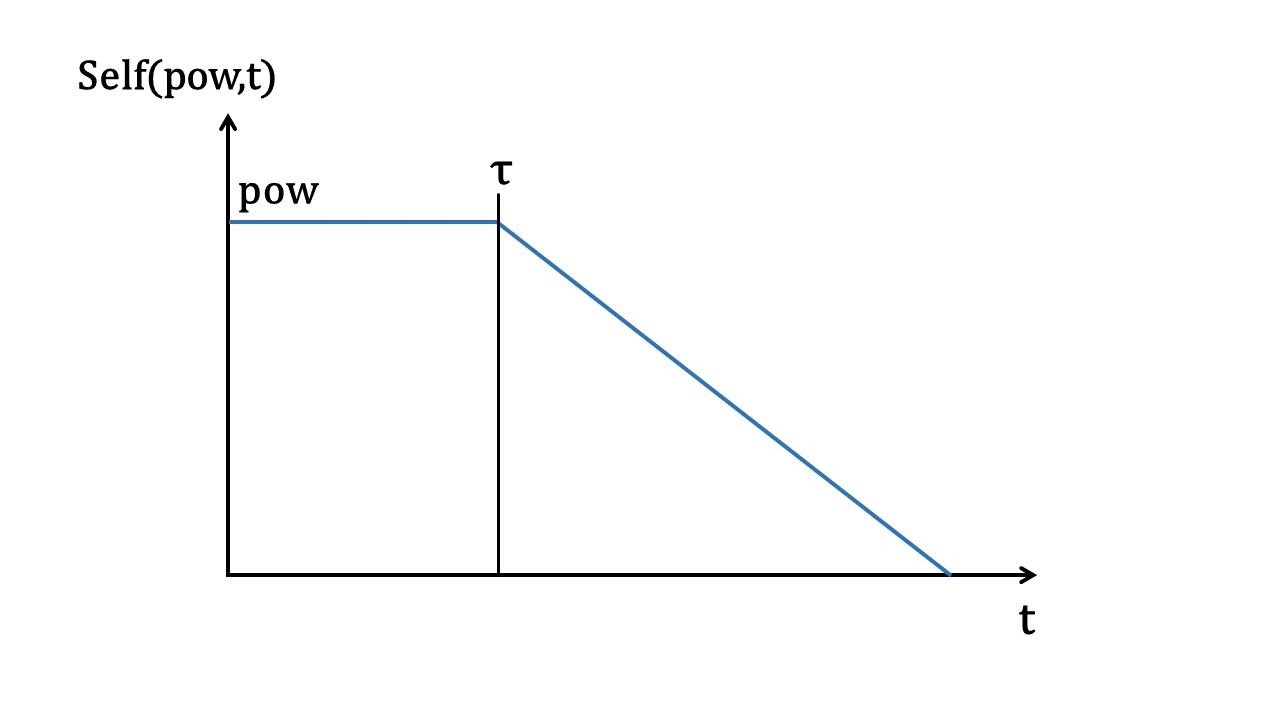
\includegraphics[width= 4 in, height = 2 in]{graphs/sv3.png}
		\caption{\label{fig:conc} Concession curve. $\tau$ is a parameter that controls the moment in the negotiation when concessions begin}
		\vspace{-0.35 in}
	\end{figure} 
	%\footnote{For detailed explanation, please refer to the article \cite{ouali2017computational}}
	%illustrated in \ref{fig:conc}
	
	%	\begin{equation}
	%	self(pow, t) = \left\{\begin{array}{ll}
	%	pow & \mathrm{if\ } (t \leq \tau)\\
	%	max(0, pow - (\frac{\delta}{pow} \cdot (t - \tau))) & \mathrm{otherwise}
	%	\end{array}\right.
	%	\end{equation}
	
	
	The level of demand shows up in negotiation when the agent has to decide wheather a proposal is acceptable.
	Therefore, we implemented a function that computes the acceptability of proposals. Let be $v$ a proposal, thus its acceptability is computed:
	
	\begin{equation}
	acc(pow,v, t) = sat_{self}(v, \prec_i) \geq   self(pow,t)
	\end{equation}
	
	
	\subsubsection{Self vs other:} Low-power negotiators consider the preferences when making decisions, whereas high-power negotiators are self-centered and only interested in satisfying their own preferences. \cite{fiske1993controlling,de1995impact}.
	Therefore, when the agent makes proposals, it has to take into account its preferences and its interlocutor's preferences with respect of the weight it gives to the satisfaction of its preferences and the other preferences.	
	Let us consider the subset $V_i\subseteq C_i$ of values that are acceptable for the agent:
	%\vspace{-0.5em} 
	\begin{equation}
	V_i(pow,t) = \{ v\in C_i : acc(pow,v,t) \}
	%	\vspace{-0.5em}
	\end{equation}
	
	We propose a function for a proposal selection as follows:
	\begin{equation}
	\begin{split}
	tol(v, t, \prec_i, A_i, U_i, pow) & = self(pow, t) . sat_{self}(v, \prec_i) \\
	& +  (1 - self(pow, t)) . sat_{other}(v, A_i, U_i)
	\end{split}
	\end{equation}
	
	\subsubsection{Controlling the flow of the negotiation:}
	High-power negotiators tend to make the first move \cite{magee2007power} and take the lead in the negotiation. Low-power negotiators aim to construct an accurate model of other preferences, which leads them to ask more questions about other preferences rather than keeping the negotiation going (\emph{e.g} by making proposals)\cite{de2004influence}.
	The lead of the negotiation is reflected throughout the utterances expressed during the negotiation. Therefore, we defined rules that control the choice of the utterance and reflects the cited behaviors. A high-powerful agent will try to keep the negotiation going by priorizing \emph{Negotiation moves} (see section \ref{Comm}). In addition, we designed additional utterances (\textit{i.e} \emph{RejectPropose, AcceptPropose}) allowing the agent to express the control of the negotiation.
	In the contrary, low power agent will at first, focus on \emph{information moves} in order to learn more about the preferences of its interlocutor then make proposals that suits the knowledge gathered. 
	The details of the algorithm are presented in \cite {ouali2017computational}
	
	\section{Experiment}
	We conducted a study to evaluate the negotiation model during interactions with human users. We aim to analyze the user's perception of the agent behavior during the negotiation.
	
	\subsection{Study design}
	
	Participants negotiate with the agent on the social topic of \emph{"restaurants"}. Our aim was to define a social topic which does not require specific expertise and participants have personal preferences.
	
	The criteria defined to choose a restaurant were \{ \textit{cuisine, price, ambiance, location}\}. Each criterion was defined with a domain of values, and a total of 420 of restaurants was generated from the values of each criterion.
	
	We defined two agents Bob and Arthur which play different behaviors. We designed Bob to follow a high power behavior (\textit{i.e} pow(Bob) = 0.8) and Arthur to play the low power negotiator (\textit{i.e} pow(Arthur) = 0.4).
	Participants interacted with agents thought a GUI (Graphical User Interface) that we designed for the experiment. They communicated using the utterances that we defined see (section \ref{Comm}). Figure \ref{ihm} shows the GUI with the possible utterances to enunciate.
	
	\begin{figure}[t]
		\centering
		\fbox{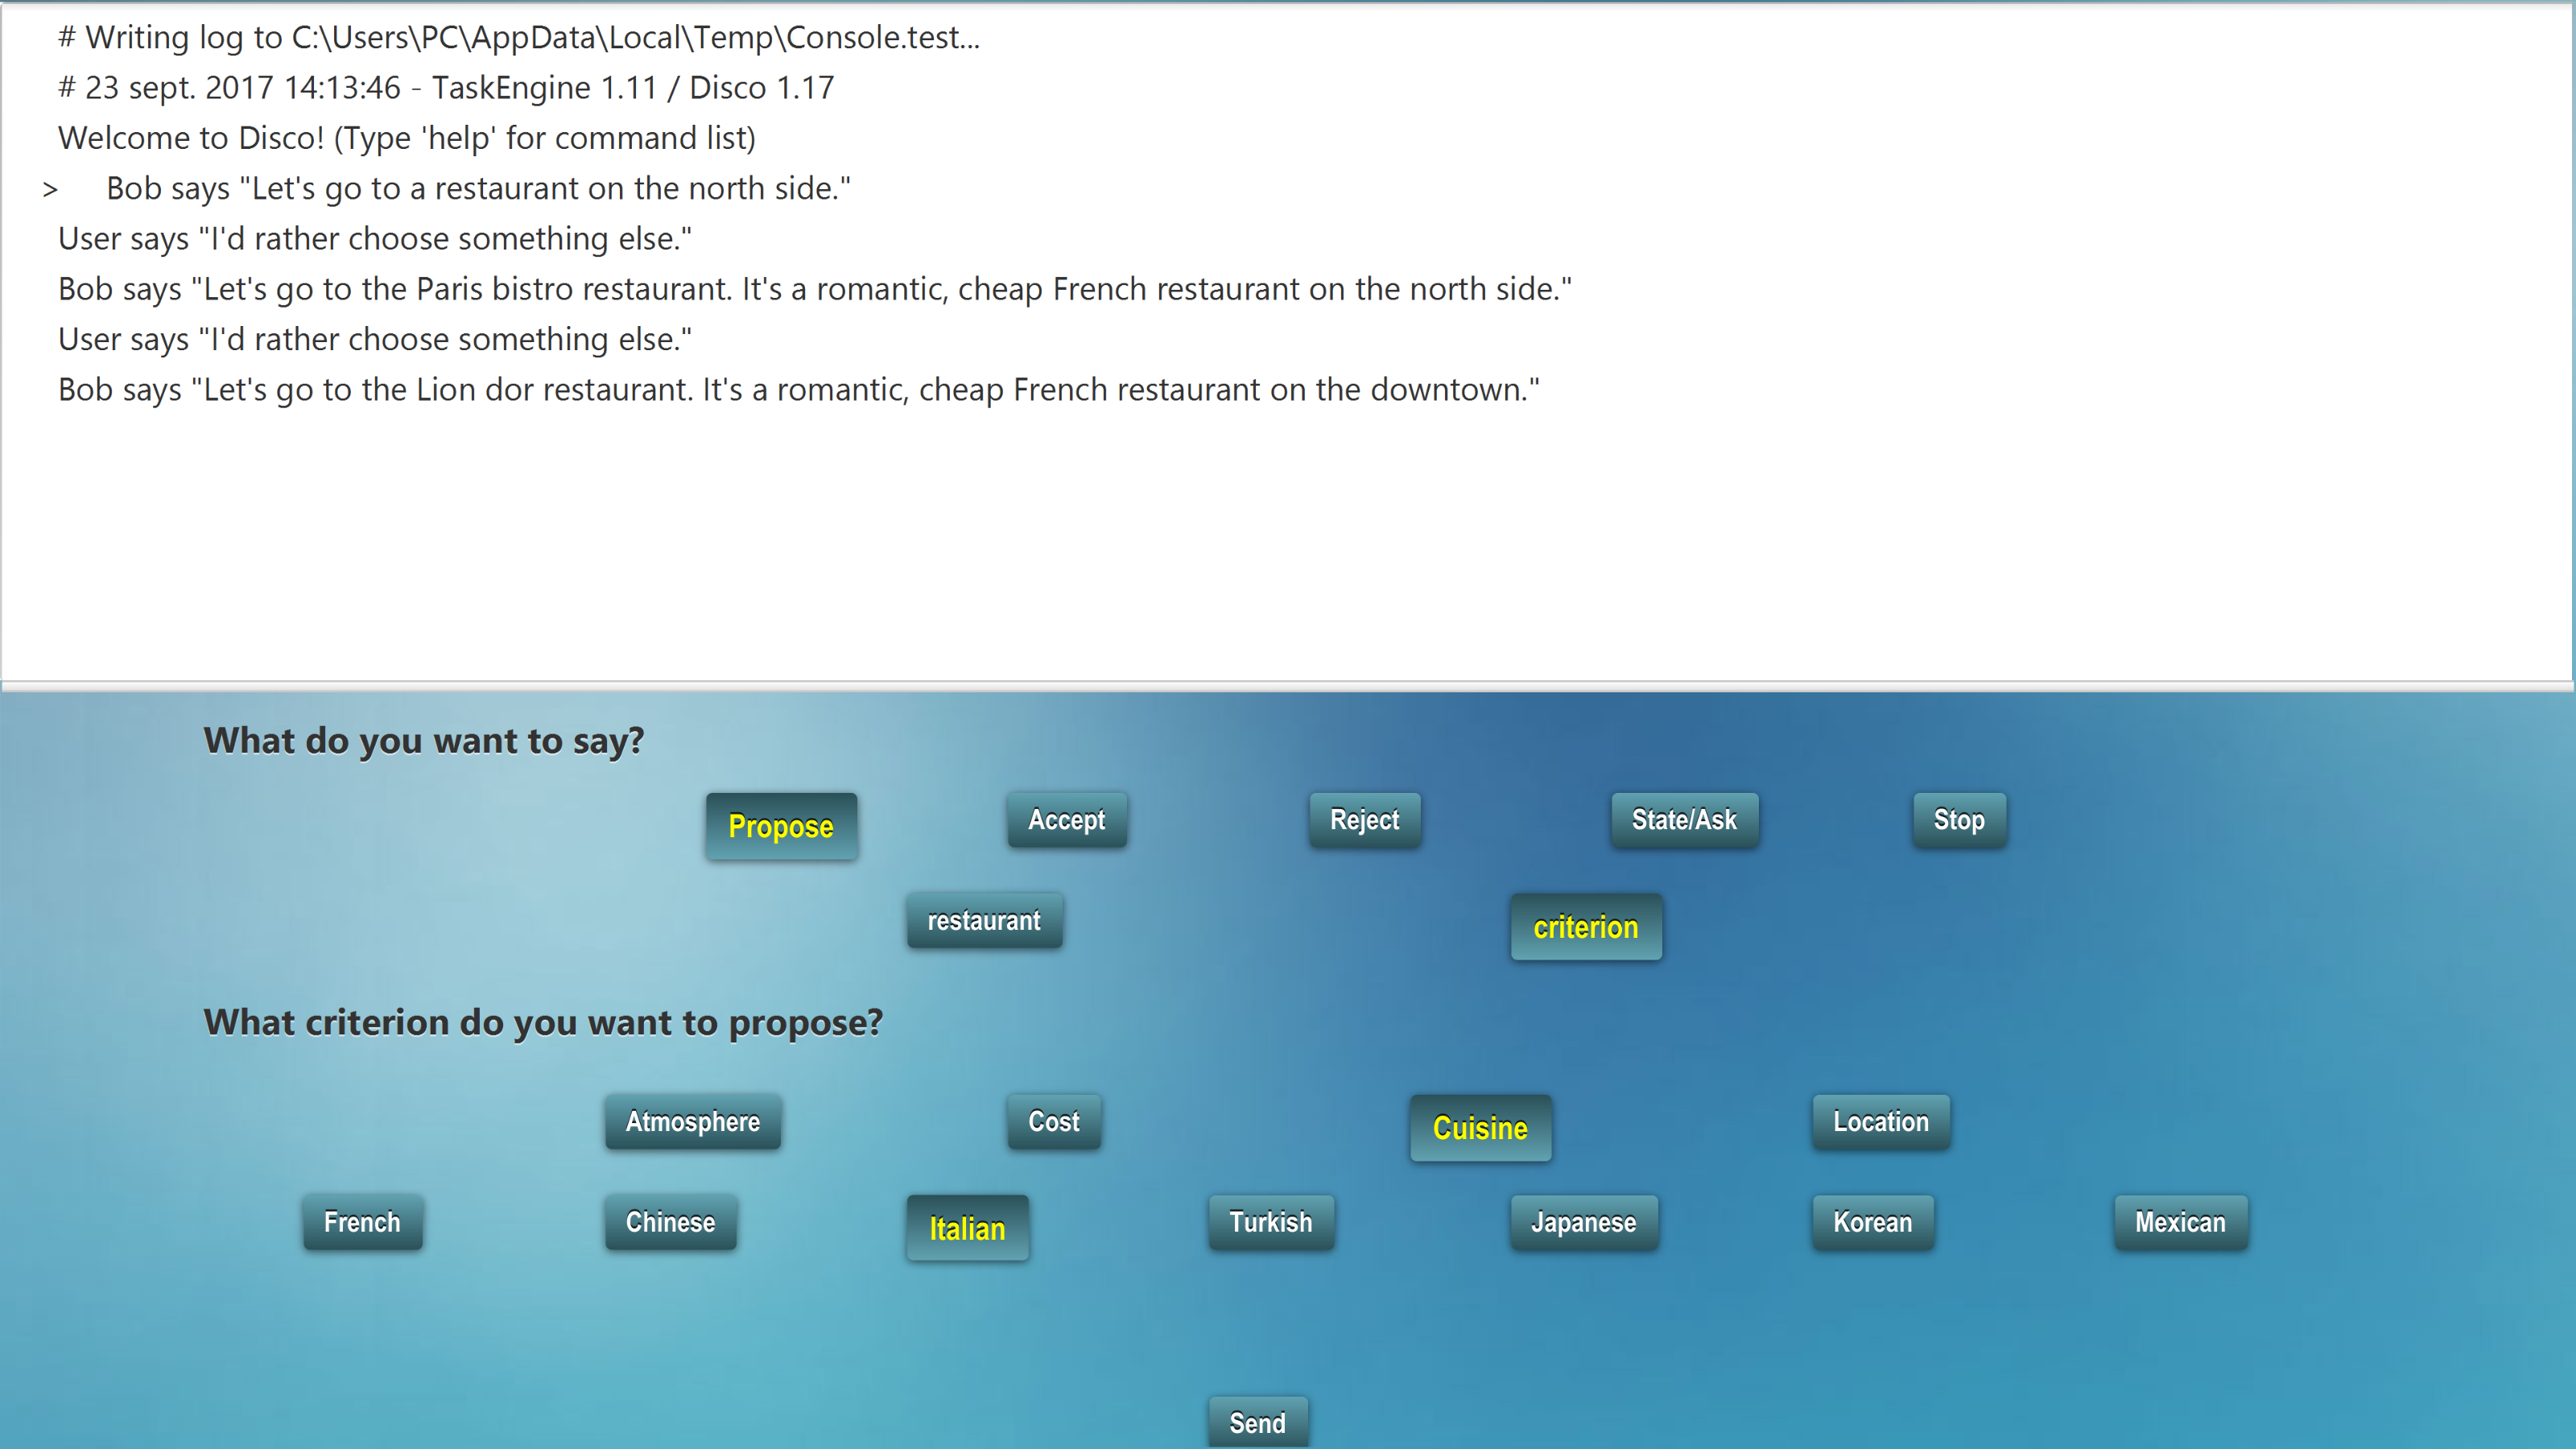
\includegraphics [width=\textwidth, height = 0.45\textheight]{graphs/ihm1.png}}
		\caption{GUI for participant. User currently selects the utterance Propose(Italian), which corresponds to the verbal utterance:  ''Let's go to an Italian restaurant.''}
		\label{ihm}
	\end{figure}
	
	We defined two experimental designs in order to not bias the perception of participants. In the first one, participants interacted first with Bob, the hight power agent, following the interaction with the low power agent Arthur. In the contrary, the second condition, participants interacted first with Arthur then with Bob. 
	
	\subsection{Hypotheses}
	We defined four hypotheses that reflect the different behaviors and strategies displayed by agents when negotiating.
	
	\begin{itemize}
		\item  \textbf{H1:} The higher-power agent will more strongly be perceived as self-centered than the lower-power agent.  
		
		\item \textbf{H2:}  The higher-power agent will more strongly be perceived as demanding than the lower-power agent.
		
		\item \textbf{H3:} The lower-power agent will be more strongly perceived as making larger concessions than the higher-power agent.
		
		\item \textbf{H4:}  The higher-power agent will more strongly be perceived as taking the lead in the negotiation than the lower-power agent.
		
	\end{itemize}
	
	\subsection{Experimental Procedure}
	We conducted a within-subject where each participant interacted with both  agents Bob and Arthur.
	
	Upon arrival, the participant is asked to sign an informed consent form and the negotiation task was explained. Following this, training session begins, the participant is given instruction on the use of the GUI to interact with the agent, the experimenter starts the training session and leaves the room until training is complete and the participant is familiar with the interface. Following training, the experiment begins and the participant negotiates with the agents. Upon completion of the negotiation, the participant is asked to fill out a questionnaire about his experience.
	
	We designed a questionnaire allowing the participants to report his perception of the agent's behaviors during the negotiation. For each hypothesis, we defined two questions with different formulations in order to not bias the answers of participants. In addition, we defined test questions to check the sanity of the participant's answers. The responses are given on Likert scale.
	
	
	A total of 40 participants participated in the experiment. They were randomly assigned to the experimental conditions.% We balanced the population for each condition. 
	
	\subsection{Results}
	
	
	Our analysis first checked the perception of the agent behaviors during the interaction. The results are summarized in figure \ref{res}.
	
	Participants have perceived that agent bob leads the negotiation (\emph{M= 4.40, SD= 0.9}). They also rated bob to be demanding (\emph{M= 3.59, SD= 1.3}) and not self-centered (\emph{M =2.92, SD =1.3}). In addition, to the questions about concessions made during the negotiation, participants perceived that bob make few concessions (\emph{M=3.29, SD =1.24}).
	
	In the contrary, participants perceived the behavior of Arthur as follows: In average, Arthur doesn't lead the dialogue (\emph{M= 1.76, SD= 1.09}). It has a low level of demand (\emph{M= 2.32, SD= 1.3}) and makes few concessions (\emph{M= 3.39, SD= 1.16}). Furthermore, Arthur was perceived as taking into account the participant preferences and is not selfish (\emph{M=2.7, SD =1.13}).
	
	The second step of our analysis concerns the evaluation of both agents behaviors. We compared the behavior of Bob and Arthur using a \textit{non parametric Wilcoxon signed-rank test}. Our first hypothesis predicted that the high power agent Bob would be perceived as more self-centered than low power agent Arthur. Our analysis confirmed our prediction; participants perceived Bob to be more self-centered than Arthur (\emph{Z=-3.2, p = 0.001, d= -0.3}). In addition, our second hypothesis was also confirmed. Bob was perceived as being more demanding than Arthur with a small effect size(\emph{Z=-3.6, p < 0.001, d=-0.3}). 
	
	The third hypothesis predicted that Arthur would make larger concessions than bob. However, the analysis of our data did not confirmed the hypothesis. There was no significant difference perceived in concessions made by agents during the negotiation (\emph{Z=-3.2, p = 0.001, d=-0.05}).
	
	The last hypothesis was confirmed. The Wilcoxon ranked test revealed that Bob agent was perceived as significantly more leading the dialogue than Arthur, with a medium effect size (\emph{Z=-3.2, p = 0.001, d= -0.6}).
	%	\vspace{-.9em}  
	\begin{figure}[h]
		\centering
		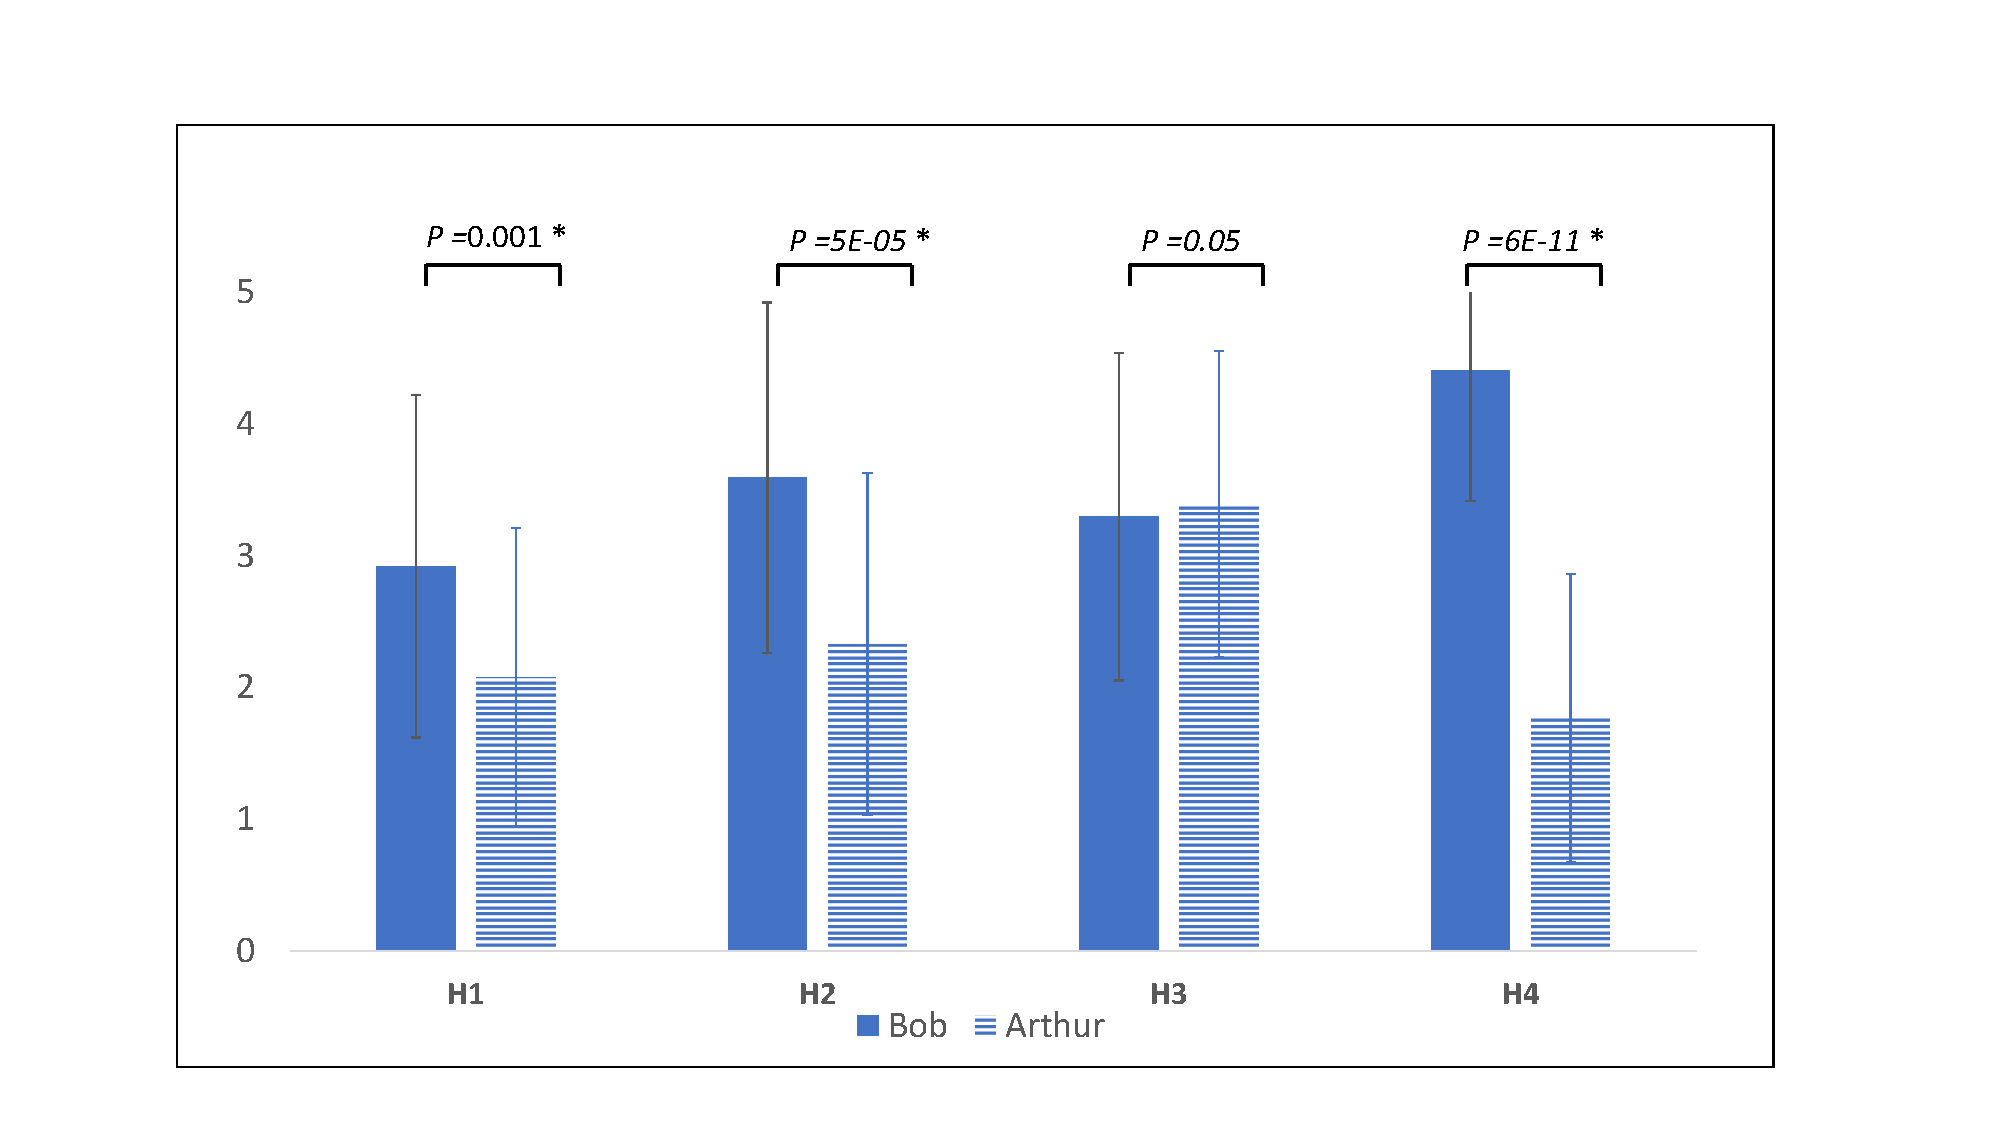
\includegraphics[width=\textwidth,height=0.42\textheight]{graphs/res.pdf}
		\caption{The results from our analysis}
		\label{res}
	\end{figure}
	%	\vspace{-.5em} 
	
	\subsection{Discussion}
	
	The results of our experiment provide strong support for three out of four hypotheses. Participants perceived Bob the high power agent to lead the negotiation, to be self-centered and more demanding compared to Arthur, the low power agent. These results are in line with the Dedreu, Van kleef and colleagues \cite{de1995impact,de2004influence,de2004influence}  on the impact of power on the expression of negotiation strategy.  
	
	However, our third hypothesis was not confirmed as participants did not perceive a significant difference in the level of concessions expressed by Bob and Arthur. This result can be explained by the impact of preferences on the outcome of the negotiation. Preferences affect the strategy displayed by the agent. In the case where agent and user share common preferences, the negotiation will converge quickly and no confrontation of preferences will be experienced during the negotiation. This is a limitation of our experiment. We did not collect prior knowledge about the preferences of participants. Therefore, we were not able to measure the distance between the preferences of the agent and the user and to analyze the impact of preferences in the on the level of concessions.
	Therefore, we were not able to analyze the responses to hypothesis 3 to report whether concessions were only influenced by preferences or the relation of power.
	
	\section{Conclusion}
	
	We have presented in this paper a conversational agent able to hold a collaborative negotiation with a human user and deploy different strategies influenced by its relation of power. Agent behavior was inspired from works in social psychology that investigated how power influenced the negotiator's behaviors.
	
	The system has been tested with an interactive experiment. Participants interacted with two agents displaying different behaviors (\textit{i.e.} high power behavior and low power behavior).
	
	The results have important implications for the design of artificial agents that can negotiate with people. Artificial intelligence research in automated negotiation has focused on different aspects of the task of negotiation such as the number of issues discussed, the parties implied in the negotiation, and so on. However, fewer research investigates the impact of the social context \cite{de2011effect,nazari2015opponent}. This work is a continuation of this field, where we aim to demonstrate the importance of social behaviors when implementing agents that interact with a human. %We focus on the impact of interpersonal relation of dominance in the agent negotiation strategy.
	
	The next step of our research is to study the construction of the relation of dominance during the negotiation and its impact on both the strategies displayed by the negotiators as well as the outcomes of the negotiation.
	
	% ================== BIBLIO ===============
	
	\scriptsize{	
		\bibliographystyle{splncs}
		\bibliography{Library}}
	
\end{document}